\begin{figure}[H]
\centering
\shorthandoff{<>}
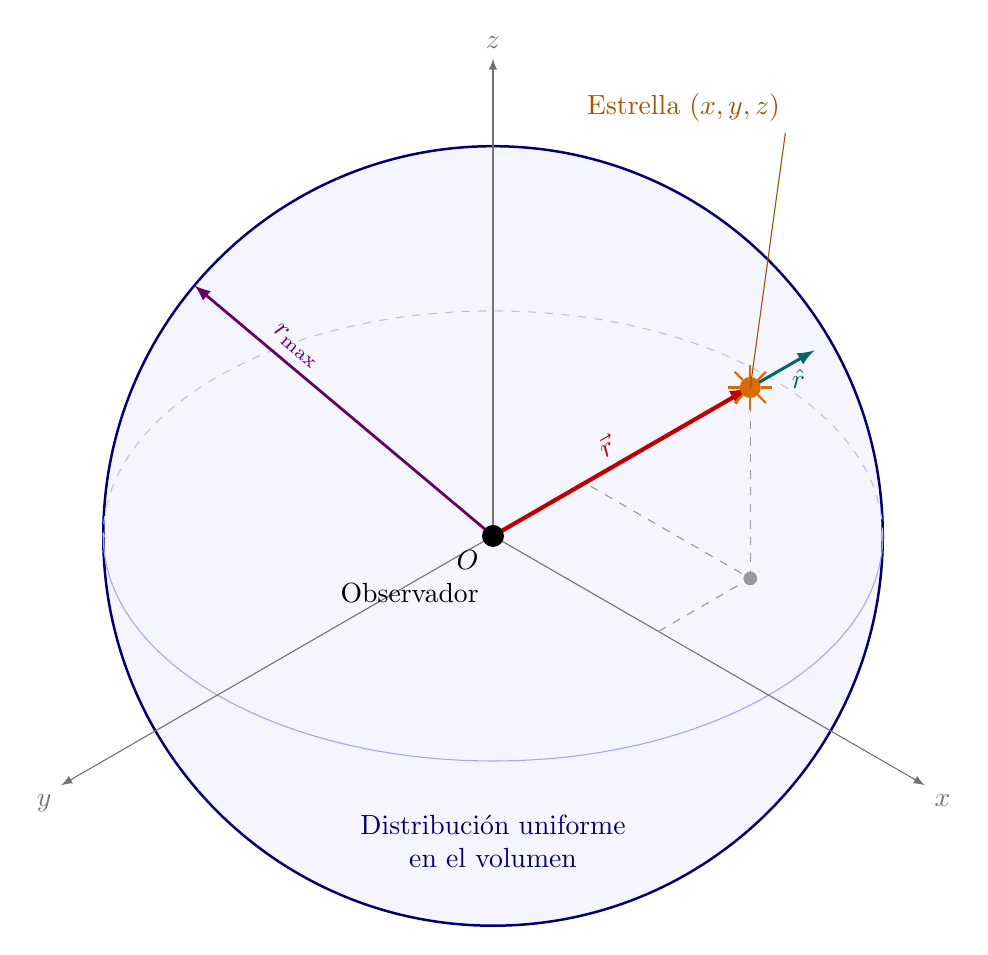
\begin{tikzpicture}[scale=1.65,font=\normalsize,>=latex]
  \fill[blue!4] (0,0) circle (3cm);
  \draw[blue!45!black,line width=0.9pt] (0,0) circle (3cm);
  \draw[blue!25,dashed] (3,0) arc[start angle=0,end angle=180,x radius=3cm,y radius=1.732cm];
  \draw[blue!35] (-3,0) arc[start angle=180,end angle=360,x radius=3cm,y radius=1.732cm];

  \begin{scope}[x={(0.7071cm,-0.40825cm)},y={(-0.7071cm,-0.40825cm)},z={(0cm,0.8165cm)}]
    \coordinate (observer) at (0,0,0);
    \coordinate (star) at (1.8,-1,1.8);
    \coordinate (planar) at (1.8,-1,0);
    \coordinate (xcomponent) at (1.8,0,0);
    \coordinate (ycomponent) at (0,-1,0);
    \coordinate (radialtip) at (2.25,-1.25,2.25);
    \draw[->,black!55] (0,0,0) -- (4.7,0,0) node[below right] {$x$};
    \draw[->,black!55] (0,0,0) -- (0,4.7,0) node[below left] {$y$};
    \draw[->,black!55] (0,0,0) -- (0,0,4.5) node[above] {$z$};
  \end{scope}

  \draw[dashed,black!40] (star) -- (planar);
  \draw[dashed,black!40] (xcomponent) -- (planar) -- (ycomponent);
  \fill[black!40] (planar) circle (1.5pt);

  \draw[->,violet!80!black,line width=1pt] (observer) -- (140:3)
    node[pos=0.7,above,sloped] {$r_{\max}$};
  \draw[->,red!75!black,line width=1.5pt] (observer) -- (star)
    node[pos=0.48,above,sloped] {$\vec r$};
  \draw[->,teal!80!black,line width=1.1pt] (star) -- (radialtip)
    node[pos=0.75,below,inner sep=3pt] {$\hat r$};

  \begin{scope}[shift={(star)}]
    \foreach \angle in {0,45,90,135,180,225,270,315}{
      \draw[orange!85!black,line width=0.8pt] (\angle:0.08) -- (\angle:0.17);
    }
    \fill[orange!85!black] (0,0) circle (2.3pt);
  \end{scope}
  \node[anchor=west,text=orange!65!black] at (0.65,3.3) {Estrella $(x,y,z)$};
  \draw[orange!65!black,thin] (2.25,3.1) -- (star);

  \fill[black] (observer) circle (2.4pt);
  \node[below left,align=right,inner sep=5pt] at (observer)
    {$O$\\Observador};
  \node[text=blue!45!black,align=center] at (0,-2.35)
    {Distribución uniforme\\en el volumen};

\end{tikzpicture}
\shorthandon{<>}
\caption{Geometría de la esfera y elementos vectoriales del problema. El observador está en el origen; $\vec r$ localiza una estrella y $R$ es su distancia al centro. El círculo exterior representa el contorno de la esfera de radio $r_{\max}$ y la elipse representa su sección en el plano $xy$. Las líneas grises discontinuas muestran proyecciones cartesianas. La flecha $\hat r$ indica la dirección radial hacia afuera y se dibuja a una escala ilustrativa.}
\label{fig:esfera-flujo-estelar}
\end{figure}